%!TEX root = ../../../memoria.tex

\begin{figure}[H]
	\centering
	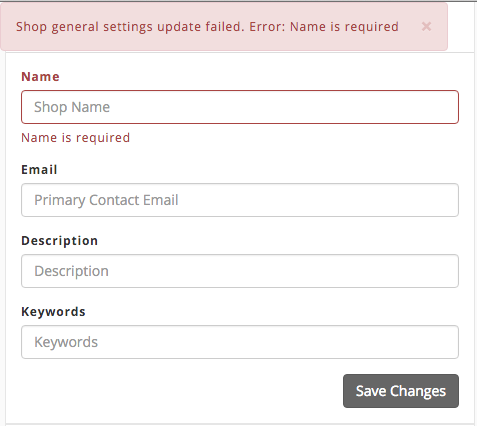
\includegraphics[width=0.6\textwidth]{figuras/dashboard/ecommerce/general_menu/updated_error.png}
	\caption{Errores en el formulario tras enviarlo. El campo \textit{Name} es obligatorio.}
	\label{figure:apendice:dashboard:ecommerce:general_menu:updated_error}
\end{figure}

\begin{figure}[H]
	\centering
	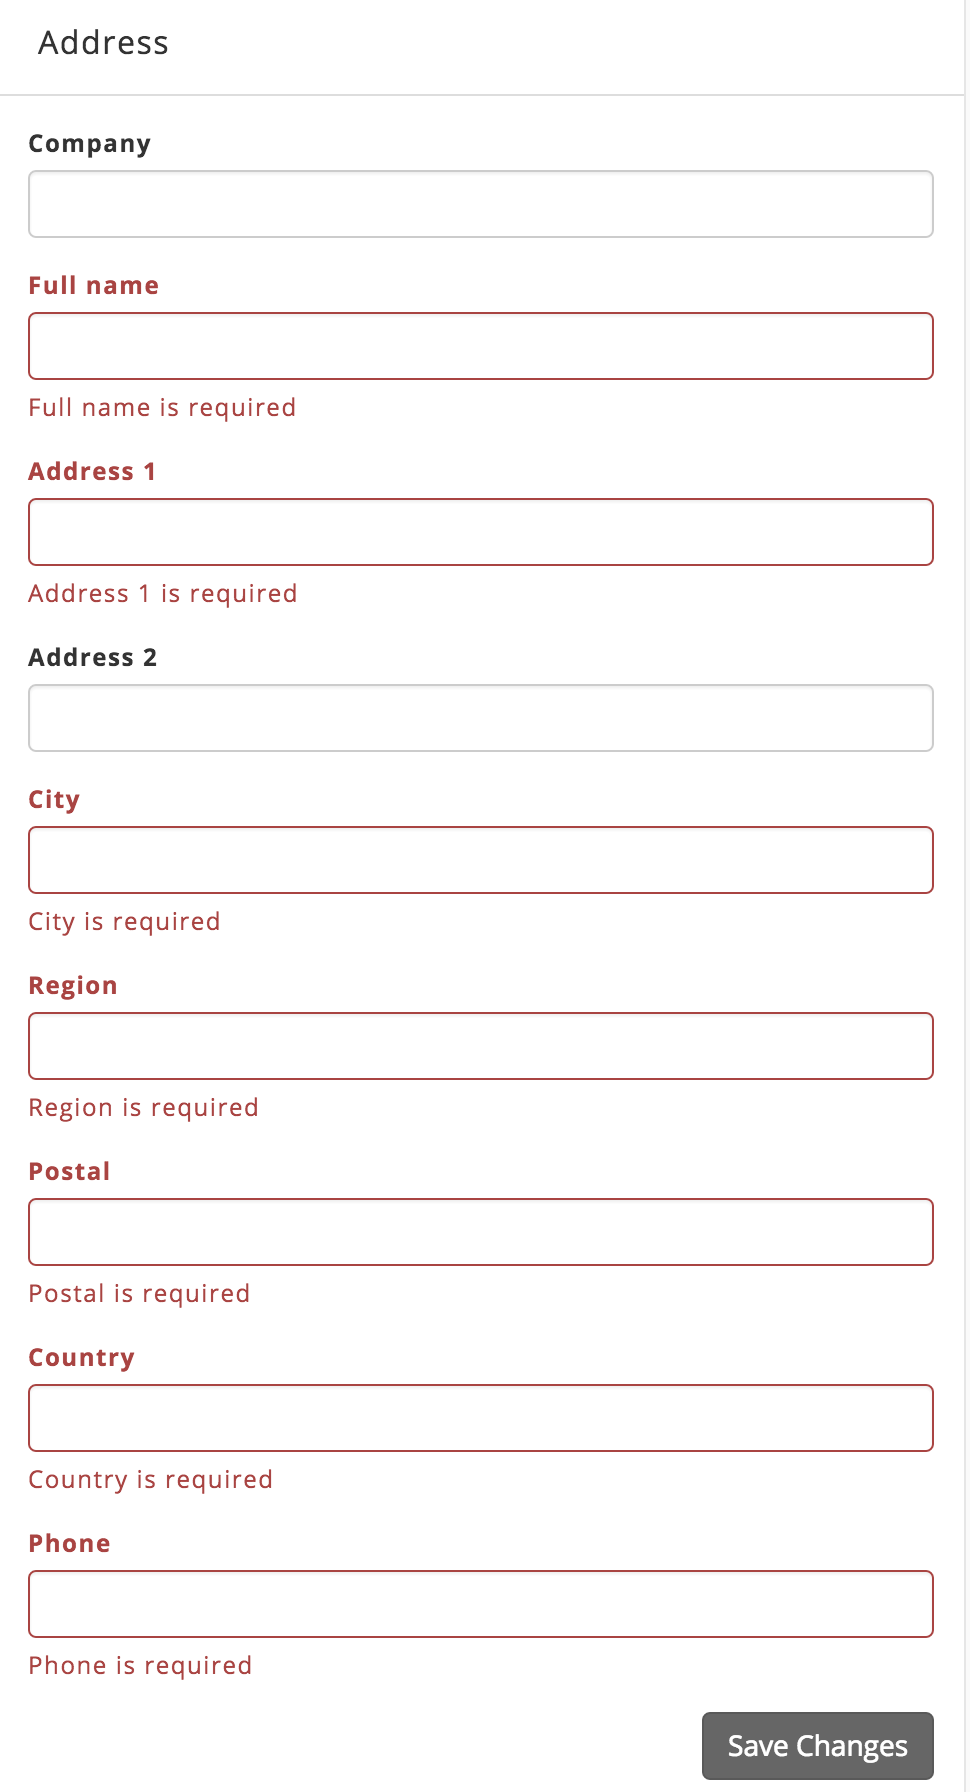
\includegraphics[width=0.5\textwidth]{figuras/dashboard/ecommerce/address/updated_error.png}
	\caption{Comentarios del formulario tras error de actualización.}
	\label{figure:apendice:dashboard:ecommerce:address:updated_error}
\end{figure}

\begin{figure}[H]
	\centering
	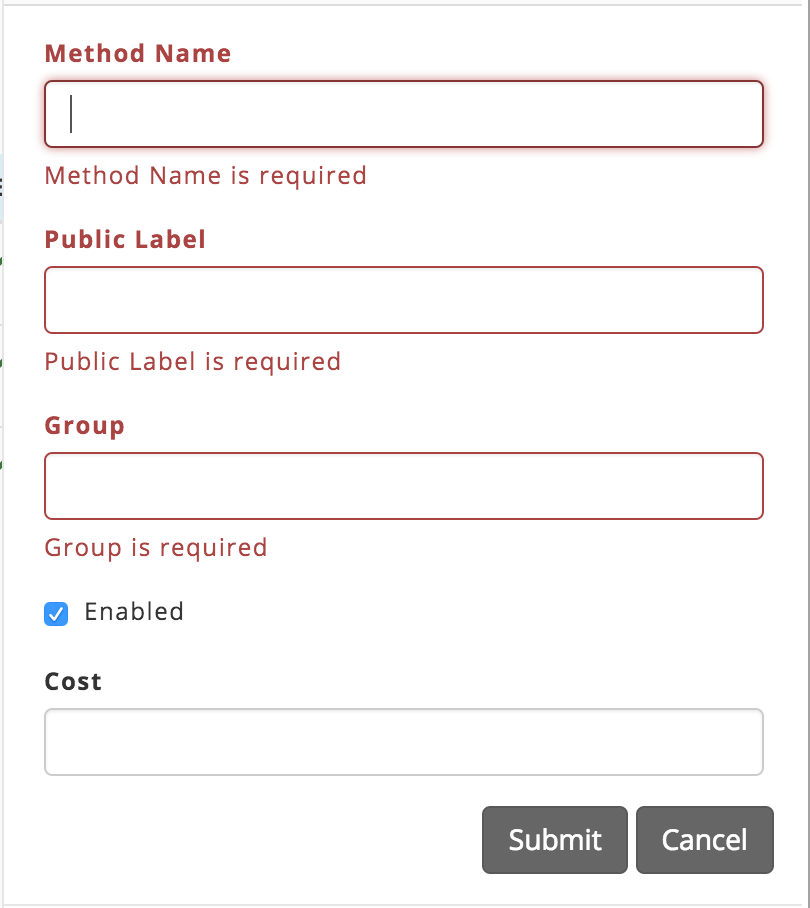
\includegraphics[width=0.6\textwidth]{figuras/dashboard/shipping/form_shipping_add_send_empty.png}
	\caption{Formulario de creación de \shippingEF tras enviarlo vacio.}
	\label{figure:apendice:dashboard:shipping:form_shipping_add_send_empty}
\end{figure}